\chapter{Экспериментальные результаты}\label{ch:ch4}

\section{Исследование алюминиевого сплава системы Al-Mg-Si}\label{sec:ch4/sect1}

После сборки и запуска ПАЗЛ-3D появилась необходимость по демонстрации возможностей установки по исследованию сплавов на основе алюминия  с наноразмерными особенностями. При этом материал должен был удовлетворять следующим требованиям. Материал - многокомпонентный сплав, имеющий хорошую теплопроводность. В нём должны присутствовать структуры с характерным размером от 10 до 100 нм. Вышеуказанные требования позволили, с одной стороны, продемонстрировать возможности установки по характеризации наноструктур и масс-спектрометрии, с другой стороны, материал позволяет максимально упростить проведение исследования, благодаря хорошей теплопроводности и электрической проводимости. Перечисленным требованиям отвечал сплав Al-Mg-Sc. Алюминиевые сплавы, в зависимости от легирующих элементов, могут обладать повышенной прочностью, пластичностью, коррозийной стойкостью, жаростойкость. Благодаря своим свойствам такие сплавы широко применяются как конструкционные материалы.
Для исследования выбранного сплава были выбраны следующие параметры исследования: температура образца 50К, мощность лазерного излучения с гармоникой 515 нм составляла 10 мВт, скорость сбора данных в ходе эксперимента лежала в пределах от 100 до 500 атомов/сек. Выбранные параметры являются наиболее часто используемые для исследования алюминиевых сплавов.
В результате проведения атомно-зондового исследования сплава были получены масс-спектр и атомные карты распределения элементов в образце. На Рисунке \cref{fig:AlMgSi_mass} представлена основная часть масс-спектра. Среднее разрешение по массе на полувысоте пика составило 500 единиц.

\begin{figure}[ht]
	\centerfloat{
		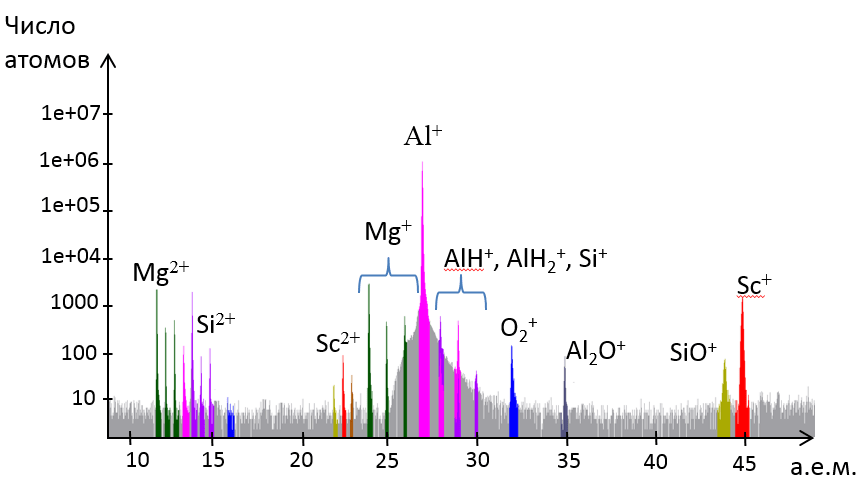
\includegraphics[scale=0.8]{AlMgSi_mass}
	}
	\caption{Основная часть масс-спектра сплава Al-Mg-Sc.}
	\label{fig:AlMgSi_mass}
\end{figure} 

Были обнаружены наноразмерные включения, обогащенные по элементам Mg, Si, O и Cu. На Рисунке \cref{fig:AlMgSi_3D} представлены изоповерхности (поверхности одинаковой концентрации) по магнию и кремнию с обогащением в 16$\%$ и атомные карты распределения магния и кремния.

\begin{figure}[htbp]
	\begin{minipage}[b][][b]{0.49\textwidth}\centering
		%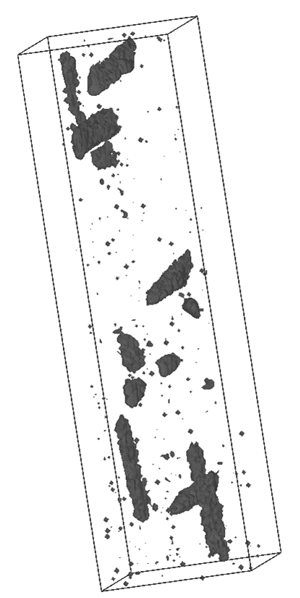
\includegraphics[width=\textwidth]{AlMgSi_3D_a} \\ а)
		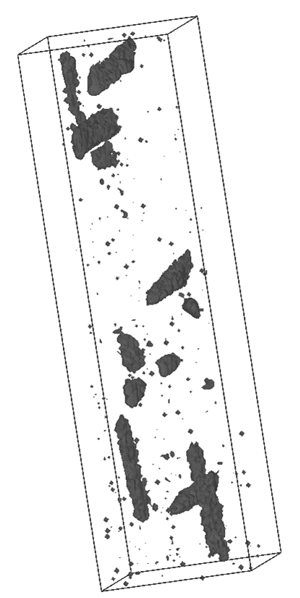
\includegraphics[scale=0.8]{AlMgSi_3D_a} \\ а)
	\end{minipage}
	%\hfill
	\begin{minipage}[b][][b]{0.49\textwidth}\centering
		%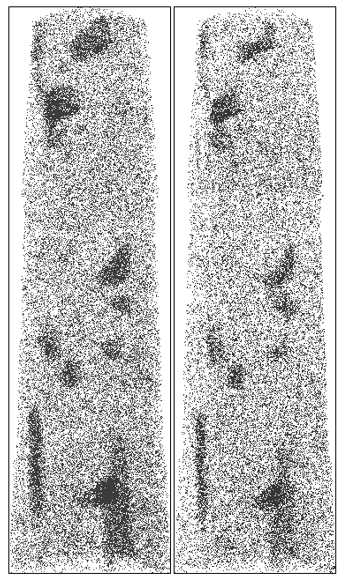
\includegraphics[width=\textwidth]{AlMgSi_3D_b} \\ б)
		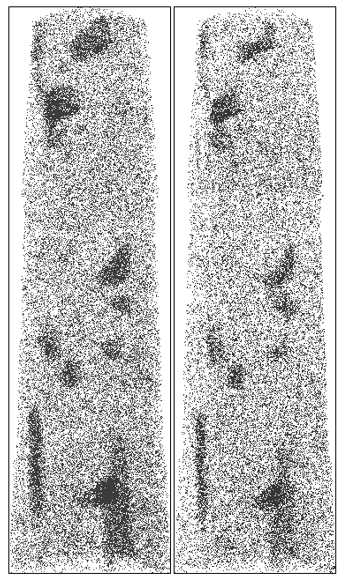
\includegraphics[scale=0.8]{AlMgSi_3D_b} \\ б)
	\end{minipage}
	\caption{а) Изоповерхность обогащения Mg и Si на 16$\%$ по сравнению с матрицей, б) атомные карты распределения магния (левый объем) и кремния (правый объем). Размер исследованной области 47х47х167 нм$^3$}
	\label{fig:AlMgSi_3D}
\end{figure} 

Обнаруженные включения имеют характерную длину порядка 50$\pm$10 нм и 10$\pm$2 нм в ширину. Размеры включений определялись по линейным размерам изоконцентрационных поверхностей. Объемная плотность составляет 2х$10^{22}$ см$^{-3}$. Ввиду несферической формы включений распределение по размерам не представляется возможным построить. Химический состав матрицы и включений показан в Таблице \cref{tab:AlMgSi_table}.

\begin{table} [htbp]
	\centering
	%\begin{threeparttable}% выравнивание подписи по границам таблицы
		\caption{Состав матрицы и включений сплава Al-Mg-Sc at $\%$}%
		\label{tab:AlMgSi_table}%
		\begin{SingleSpace}
			\begin{tabular}{| c | c | c | c | c | c | c | c |}
				\hline
				  			& Al      & Mg     & Si    & Sc     & O     & Cu     \\ \hline
				Матрица     & 98.67   & 0.56   & 0.35  & 0.31   & 0.05  & 0.03   \\ \hline
				Включения   & 67.24   & 18.22  & 13.7  & 0.36   & 0.12  & 0.36   \\ \hline				
			\end{tabular}%
		\end{SingleSpace}
	%\end{threeparttable}
\end{table}

В данной работе продемонстрирована возможность исследования сплавов на основе алюминия на установке ПАЗЛ-3D. В качестве исследуемого материала выбран сплав Al-Mg-Sc. Получены масс-спектр образца и атомные карты распределения элементов. Обнаружены включения вытянутой формы. Рассчитана объемная плотность включений и химический состав матрицы и включений. Полученные результаты подтверждают широкие возможности установки ПАЗЛ-3D по возможностям проведения исследований.

\section{Исследование алюминиевого сплава системы Al-Ca-La}\label{sec:ch4/sect2}


\section{Исследование полупроводящих материалов TiO, Si}\label{sec:ch4/sect3}